%\documentclass{sig-alternate}
\documentclass{llncs}
\usepackage{amsmath,amssymb,graphicx}
\usepackage[ruled,linesnumbered]{algorithm2e}
\usepackage{standalone}
\usepackage{algorithmic}
\usepackage{mdwlist}
\usepackage{color}
\usepackage{multirow}
\usepackage{rotating}
\usepackage{slashbox}
\usepackage{amsmath}
\usepackage[mathscr]{eucal} %% For \mathscr
\usepackage{amsbsy} %% For \boldsymbol
\newcommand{\T}[1]{\boldsymbol{\mathscr{#1}}}  
\usepackage{subfigure}
\usepackage{booktabs}
\usepackage{tikz}
\usetikzlibrary{snakes}
\usepackage{multirow}
\usepackage{epstopdf}
\usepackage{enumitem}
\usepackage{url}
\usepackage{array}
\usepackage{pdfpages}
\setlist{nolistsep}
\newcommand{\hide}[1]{}
\usepackage[labelfont=bf]{caption}
\DeclareCaptionType{copyrightbox}
\DeclareMathOperator*{\argmin}{argmin}
\DeclareMathOperator*{\argmax}{argmax}
\newcommand{\reminder}[1]{ {\color{red} {\bf  #1} } }
\newcommand{\BigO}[1]{\ensuremath{\operatorname{O}\bigl(#1\bigr)}}

\title{Binomial and Fibonacci Heaps in Racket (rkt-heaps)}

\begin{document}

\author{
	Abhinav Jauhri\\
	\texttt{abhinavjauhri@gmail.com}\\
}


% The \author macro works with any number of authors. There are two commands
% used to separate the names and addresses of multiple authors: \And and \AND.
%
% Using \And between authors leaves it to \LaTeX{} to determine where to break
% the lines. Using \AND forces a linebreak at that point. So, if \LaTeX{}
% puts 3 of 4 authors names on the first line, and the last on the second
% line, try using \AND instead of \And before the third author name.

%\newcommand{\fix}{\marginpar{FIX}}
%\newcommand{\new}{\marginpar{NEW}}

%\nipsfinalcopy % Uncomment for camera-ready version


\maketitle
%\vspace{-0.5in}

\begin{abstract}
	Library\footnote{Will be referred as $rkt-heaps$ throughout the paper} providing data structures viz. Binomial heap \cite{vuillemin1978data} and Fibonacci heap\cite{fredman1987fibonacci} are described along with primitive operations, performance and usage. 
\end{abstract}

\section{Introduction}
%\vspace{-0.1in}
$rkt-heaps$ library is made for demonstration in a contest, \textit{Lisp In Summer Projects}\footnote{http://lispinsummerprojects.org/}. The goals of any participant in the contest were to build and demonstrate a project using any LISP-based technology. $rkt-heaps$ uses Racket language belonging to the Lisp/Scheme family. \\

\emph{Section 1 \& 2} describe Binomial and Fibonacci heaps respectively. \emph{Section 3} has performance results to complement the theoretical run-time bounds. Comparison with an existing library for Binary heaps\footnote{http://docs.racket-lang.org/data/Binary\_Heaps.html} in Racket is also added for evaluation purposes. \emph{Section 4} talks about syntactics of using this library in Racket.

\section{Binomial Heaps}
Binomial heaps are a collection of heap-ordered Binomial trees with a pointer $min$ to the root of a tree having the minimum value amongst all elements in the heap. They allow the following operations: \\

\begin{enumerate}
	\item \emph{makeheap(i)} Makes a new heap with only one element \emph{i}.
	\item \emph{findmin(h)} Returns the minimum value amongst all elements in the heap.
	\item \emph{insert(h, i)} Adds element \emph{i} to heap \emph{h}
	\item \emph{deletemin(h)} Deletes the element with minimum value from \emph{h}
	\item \emph{meld(h, h')} Combines two heaps \emph{h} and \emph{h'} into one \\
\end{enumerate}

\begin{table}
	\centering
	\begin{tabular}{| >{\centering\arraybackslash}m{1in} | >{\centering\arraybackslash}m{1in} |}
		\hline
		\centering
		Operation & Amortized Cost \\ 
		\hline
		makeheap & \BigO{1}    \\
		findmin & \BigO{1} \\ 
		insert & \BigO{1}  \\
		deletemin & \BigO{\log n} \\
		meld (eager) & \BigO{\log n}\\
		meld (lazy) & \BigO{1} \\ \hline
	\end{tabular}
	\caption{Amortized costs for Binomial Heaps}
	\label{tab:binomialcost}
\end{table}

Before studying costs and implementation of the mentioned operations, some terms need brief explanations for reader's convenience. 
\begin{enumerate}
	\item $Amortized\hspace{2mm} cost$ - May not always give the exact cost of an operation. An operation may be expensive or cheaper, but the average cost over a sequence of operations is small and defined as amortized cost.
	\item $rank$ - It states the number of children of a node. For Binomial and Fibonacci heaps, only when no $decrement$ and $delete$ operations are performed, the rank of a root node is $k$ with $2^k$ nodes. \\
\end{enumerate} 

Making a new heap with one element with $makeheap$ and finding the $min$ pointer to get the minimum value with $findmin$ requires constant number of steps. Although, it may not be intuitive to see why $insert$ takes just constant amortized cost. Inserting a value is equivalent to making a heap with a single element and then merging it with the existing heap. In melding, combining two trees with same rank $k$ leads to a tree of rank $k+1$. If one already exists in either of the heaps, then a tree of rank $k+2$ is made. This happens recursively till there is single tree of some rank $(>k)$ in the resulting heap. Each time trees are combined, the heap property is imposed\footnote{Heap property ensures that all children of a tree rotted at $r$ have their values ordered with its parent's value and that the same ordering applies across the heap}. This make the average cost over $n$ operations to be \BigO{1} for $insert$. Similarly, the same idea of combining of roots of trees can be used for $deletemin$ operation. Take all children of the min root and meld them with the remaining trees in the heap, and update the min pointer, costing \BigO{\log n}.

$meld$ eager version works in the manner as described above but for the lazy version, all roots of one heap are added to the set of roots of the other heap. This may result in having more than one binomial tree of rank $k$ in the resulting heap. Any subsequent call to a $deletemin$ operation will correct the heap such that only one binomial tree of rank $k$ exists. This costs \BigO{\log n}.

Binomial heap in $rkt-heaps$ is an array-based purely functional implementation leveraging Racket's $vectors$ library. Being purely functional ensures there is no mutation of previously created data structures. Although, this leads to anomalies in runtime costs for certain operations like \emph{insert}. With reference to Table \ref{tab:binomialcost}, the total cost for $n$ inserts is linear, \BigO{n}; but in a purely functional implementation, the insert operation cost for $n$ inserts aggregates to \BigO{n^2}. The reason for such an anomaly is due to cloning of heap vector at every insert operation. This is validated in Fig:\ref{fig:bino_anomaly}. The curve \emph{binomial-insert (quadratic)} signifies the divisor(total cost) for the dividend(total time) is quadratic, and therefore the curve has slope zero\footnote{The ratio of total cost and $n^2$ will be constant}. Alternatively, taking the divisor as linear, the total run-time cost depicts a linear increase in cloning the vector, which is to say that $nth$ insertion step clones the $(n-1)th$ heap vector\footnote{Racket's vector API provides \emph{(vector-append $v_1 v_2$ \dots)}, used for cloning, makes fresh copy of all elements of given vectors}. Modifying the structuring of the heap to a doubly linked list(DDL) wherein all roots of trees have pointers to its right and left root nodes is imperative to ensure constant number of steps for each insert (used for analyzing run-time costs in \cite{kozen1992design}). The DDL implementation and cost shall be discussed in later sections of this paper. The array implementation was done out of pedagogical curiosity of the author.

\begin{figure}
	\begin{center}
		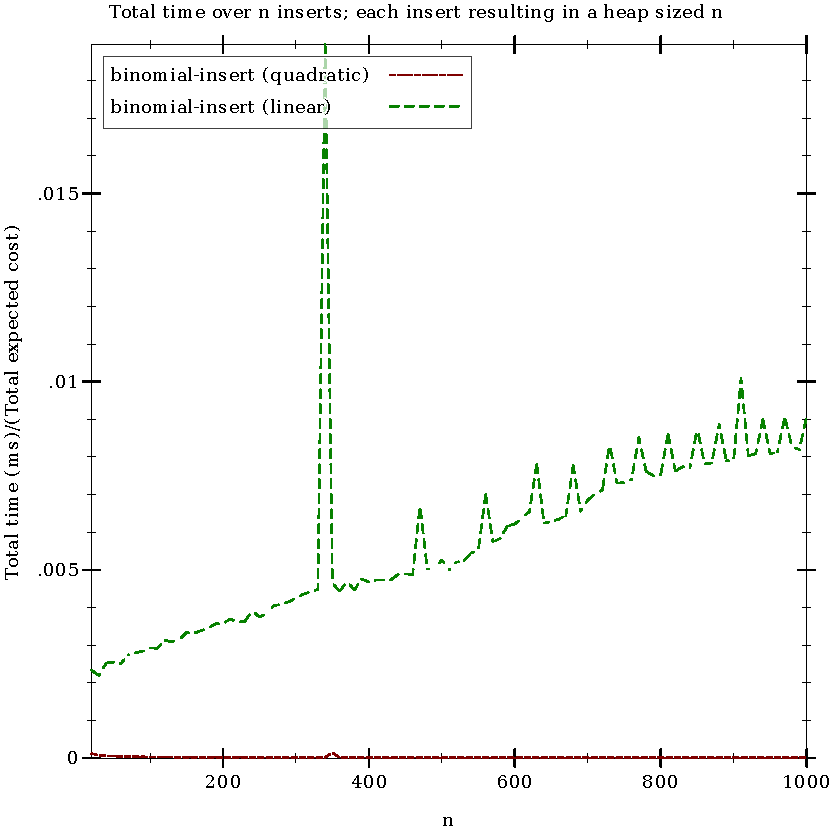
\includegraphics[width=0.8\textwidth]{FIG/insert_binomial.pdf}
	\end{center}
	\caption{Anomaly in $insert$ operations for Binomial heaps. The y-axis shows the (total runtime cost)/(total expected cost). For one curve, the total expected cost is linear in $n$, and for the other it is quadratic in $n^2$. Total time is time for $n$ insert operations and maintaining the heap state in-between each insert}
	\label{fig:bino_anomaly}
\end{figure}

\section{Fibonacci Heaps}
Fibonacci heaps are a generalization of Binomial heaps allowing additional operations other than those in Binomial heaps. Specifically, they allow deletion of an element from the heap, and modification of the value of an element. The prototypes for additional operations are as follows: \\

\begin{enumerate}
	\item \emph{decrement(h, i, $\delta$)} Decrements the value of $i$ by $\delta$ in $h$
	\item \emph{delete(h, i)} Deletes element $i$ from the heap $h$ 
\end{enumerate}

\begin{table}
	\centering
	\begin{tabular}{| >{\centering\arraybackslash}m{1in} | >{\centering\arraybackslash}m{1in} |}
		\hline
		\centering
		Operation & Amortized Cost \\ 
		\hline
		\rule{0pt}{3ex}makeheap & \BigO{1}    \\
		findmin & \BigO{1} \\ 
		insert & \BigO{1}  \\
		deletemin & \BigO{\log n} \\
		meld (lazy) & \BigO{1} \\ 
		decrement & \BigO{1} \\
		delete & \BigO{\log n}\\ \hline
	\end{tabular}
	\caption{Amortized costs for Fibonacci Heaps}
	\label{tab:fibonaccicost}
\end{table}

Fibonacci heaps are implemented in $rkt-heaps$ using a DDL for its roots. Findings from array and functional based implementation of Binomial heaps, highlight the downsides of not having mutations which leads to much higher costs for performing primitive operations in contrast to what has been proved in literature. 

As stated earlier that in a Fibonacci heap if only $deletemin$ and $meld$ operations were to be considered, then every tree becomes a binomial tree, and the heap Binomial. Thus, a corollary that the size of tree rooted at $r$ to be exponential in $rank(r)$. The exponential size of a tree is also valid for Fibonacci heaps with operations like $decrement$ and $delete$ \cite{kozen1992design}, and essential to ensure cutting of trees cost \BigO{1} and \BigO{\log n} for $decrement$ and $delete$ operations respectively. 

$decrement$ operation mutates the value of the element, followed by check on whether the heap property is violated or not. If it is, then the sub-tree rooted at that element, is added to the DDL of the heap. Every element $e$ has a flag marked as true if one of its children have been removed and false otherwise. The sub-tree rooted at $e$ shall also be cut from its parent if a second child of $e$ is removed i.e. the element is marked and a decrement operation on a child violates the heap property or a child is deleted.

$delete$ makes the value of the node to be deleted less than the min node using $decrement$ and then calls $deletemin$. This costs \BigO{\log n}.


\section{Evaluation}
For the evaluation section, we will omit comparisons between Binomial and Fibonacci heaps since one is purely functional and other is not. The functional is bound to increase the cost of operations as shown above. It is trivial to build on the Fibonacci heap implementation by excluding the $decrement$ and $deletemin$ operations to get a Binomial heap with lazy melds\cite{kozen1992design} at the same cost as shown for Fibonacci heaps in this section.

\begin{figure}
	\begin{center}
		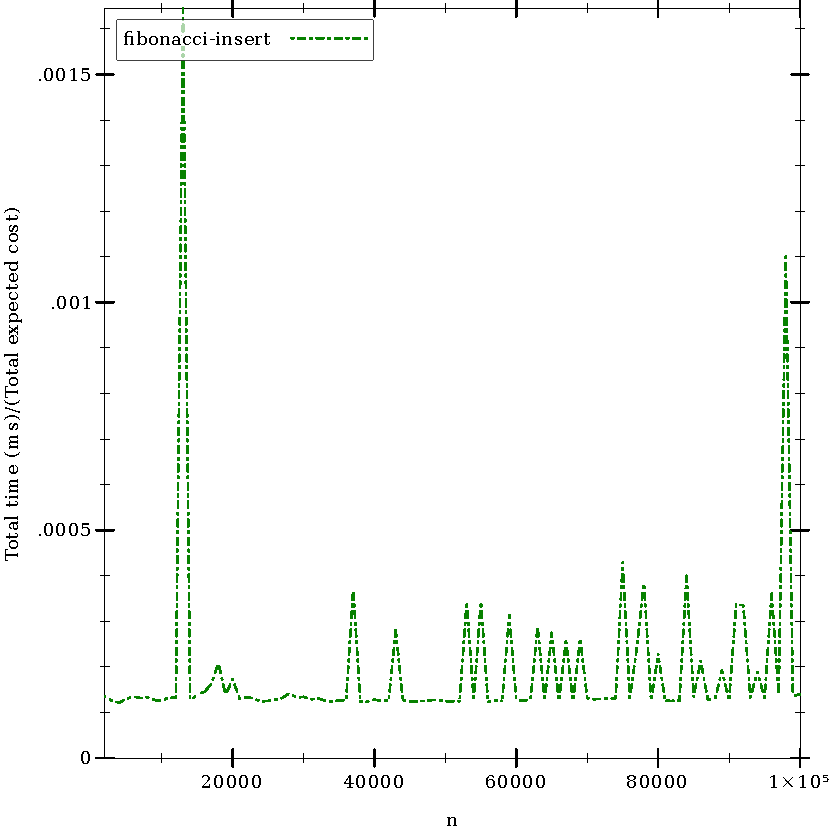
\includegraphics[width=0.8\textwidth]{FIG/insert.pdf}
	\end{center}
	\caption{}
	\label{fig:fi_insert}
\end{figure}

\begin{figure}
	\begin{center}
		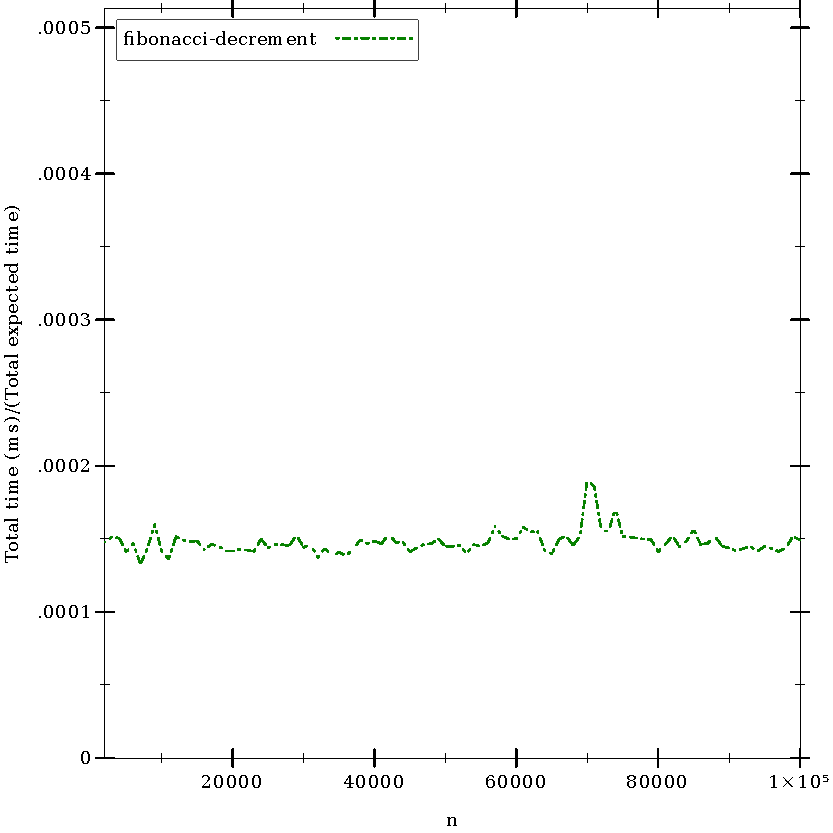
\includegraphics[width=0.8\textwidth]{FIG/decrement.pdf}
		\caption{$decrement$ operation has a expected total cost of \BigO{n}. The graph looks like a mountain terrain because we are looking at amortized version of costs.}
		\label{fig:fi_decrement}
		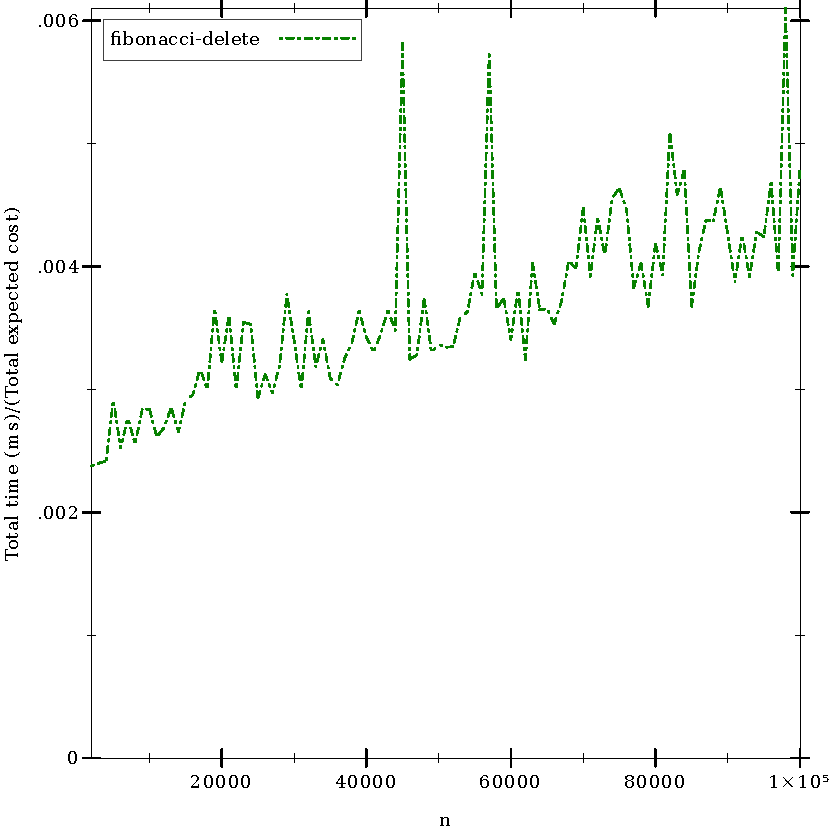
\includegraphics[width=0.8\textwidth]{FIG/delete.pdf}
		\caption{$delete$ operation has an expected total cost of \BigO{n \log n}. The sudden increase in the cost at $n=70\times10^3$ could be due the increase in the constant \# of steps by $decrement$ operation overwhelming the $\log$ \# of steps by $deletemin$ }
		\label{fig:fi_delete}
	\end{center}
\end{figure}



Binary heaps created using binary trees are compared with Fibonacci implementation of $rkt-heaps$ on operations which have equal time bounds viz. $deletemin$ and $findmin$.

deletemin for two (deletemin)
meld for one 
findmin for two (findmin)

decrement for one
delete for one

\section{Usage}
This section describes usage of $rkt-heaps$ in Racket. Clone the repository using: 
\begin{verbatim}
git clone git@github.com:ajauhri/rkt-heaps.git 
\end{verbatim}

Open Racket in terminal or add to source using:
\begin{verbatim}
(require "$RKT_HEAPS_HOME/src/binomial.rkt")
(require "$RKT_HEAPS_HOME/src/fibonacci.rkt")
\end{verbatim}

, where \$RKT\_HEAPS\_HOME is the root directory for the downloaded source.

\subsection{Binomial Heaps in Racket}
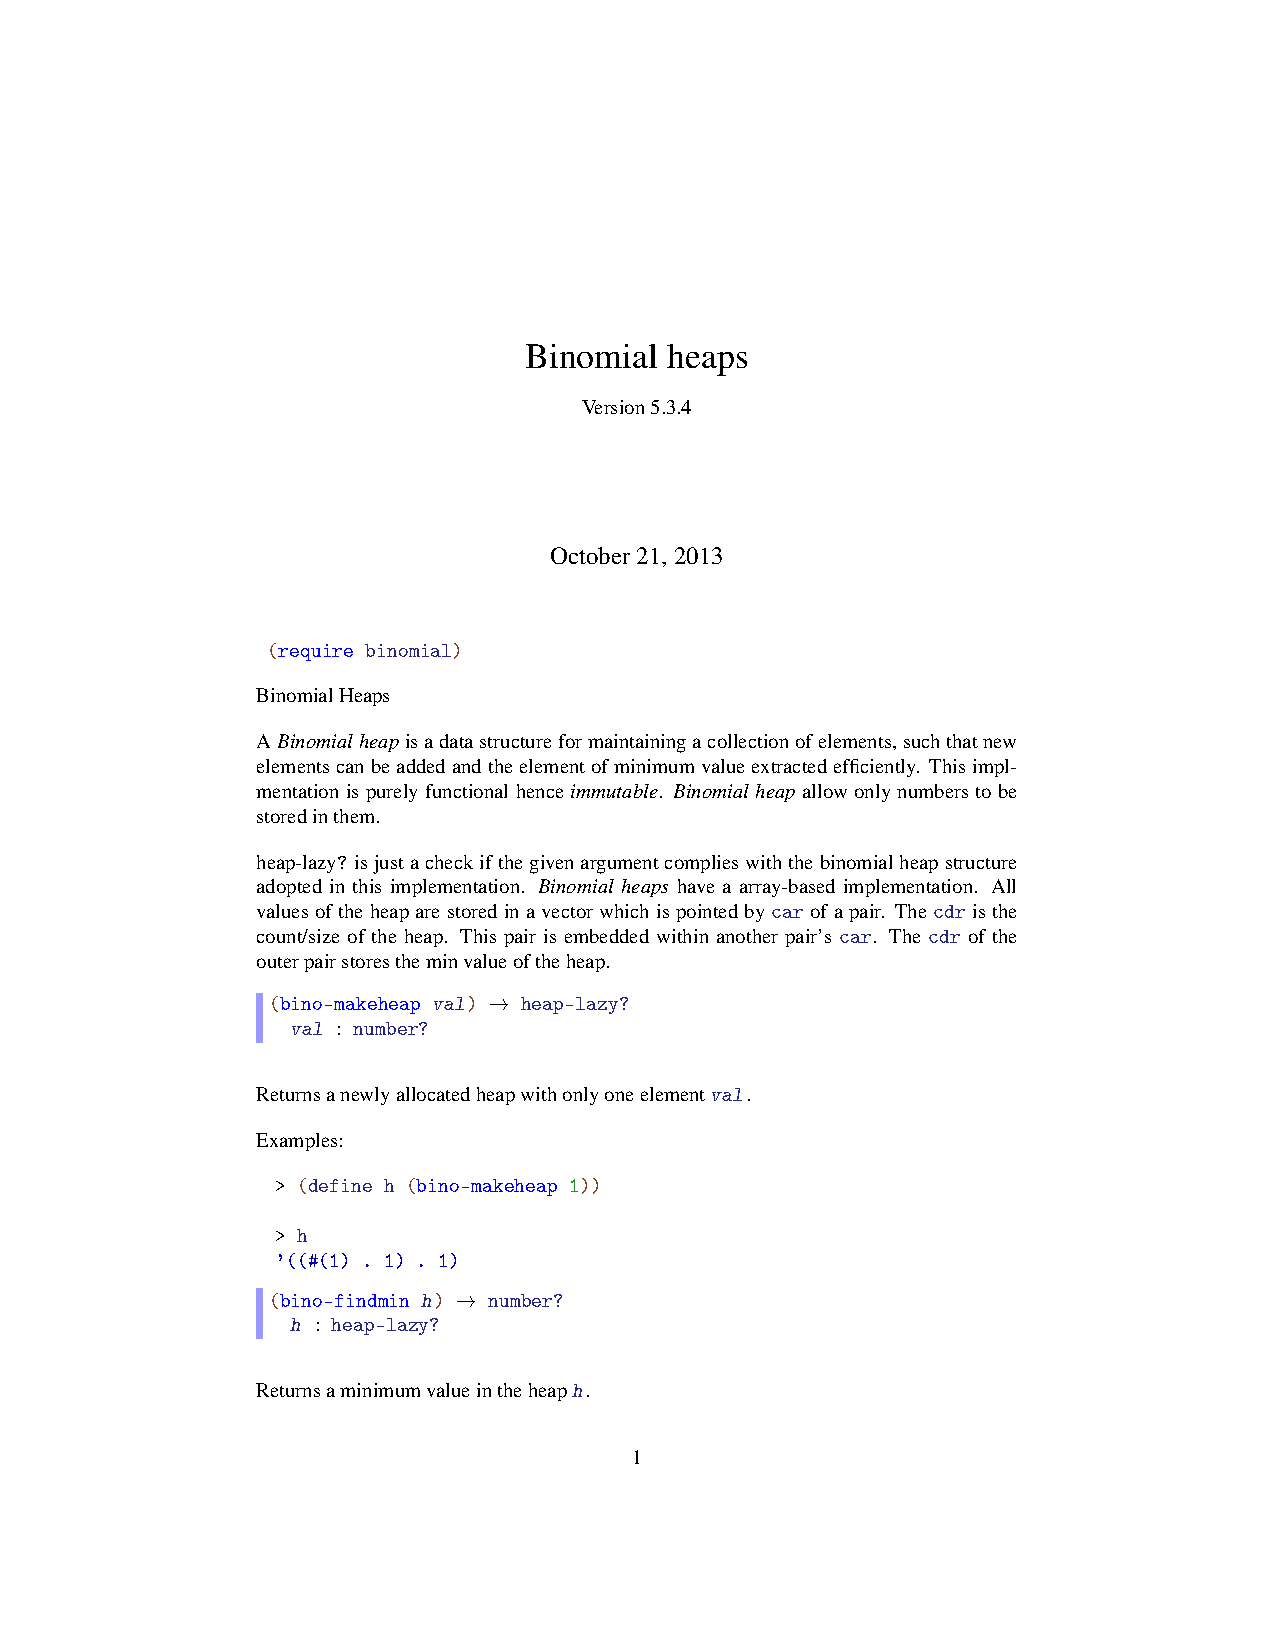
\includepdf[pages={-},nup=2x1]{../src/binomial.pdf}

\section{Conclusion}

%\newpage
\bibliographystyle{plain}
\bibliography{BIB/refs.bib}

\end{document}
